\documentclass[12pt]{article}

% ── Packages ────────────────────────────────────────────────────────────────
\usepackage[margin=1.2in]{geometry}
\usepackage{amsmath, amssymb}
\usepackage{booktabs}
\usepackage{array}
\usepackage{longtable}
\usepackage{tabularx}
\usepackage{xcolor}
\usepackage{titlesec}
\usepackage{enumitem}
\usepackage{hyperref}
\usepackage{microtype}
\usepackage{parskip}
\usepackage{fancyhdr}
\usepackage{mdframed}
\usepackage{multirow}
\usepackage{colortbl}
\usepackage{tikz}
\usetikzlibrary{arrows.meta, positioning}

% ── Colours ──────────────────────────────────────────────────────────────────
\definecolor{darkblue}{HTML}{1F3864}
\definecolor{midblue}{HTML}{2E75B6}
\definecolor{lightblue}{HTML}{D6E4F0}
\definecolor{altrow}{HTML}{EBF3FB}
\definecolor{mod1}{HTML}{EBF3FB}
\definecolor{mod2}{HTML}{EAF4EA}
\definecolor{mod3}{HTML}{FEF9E7}
\definecolor{midrow}{HTML}{F5F5F5}
\definecolor{examrow}{HTML}{F9EBEA}
\definecolor{presentrow}{HTML}{EBF5EB}

% ── Section formatting ───────────────────────────────────────────────────────
\titleformat{\section}
  {\Large\bfseries\color{darkblue}}{\thesection.}{0.6em}{}
  [\vspace{-4pt}\textcolor{midblue}{\rule{\linewidth}{0.8pt}}\vspace{2pt}]
\titleformat{\subsection}
  {\large\bfseries\color{midblue}}{\thesubsection}{0.6em}{}
\titleformat{\subsubsection}
  {\normalsize\bfseries\color{darkblue}}{\thesubsubsection}{0.6em}{}
\titlespacing{\section}{0pt}{18pt}{6pt}
\titlespacing{\subsection}{0pt}{12pt}{4pt}
\titlespacing{\subsubsection}{0pt}{8pt}{2pt}

% ── Header / footer ──────────────────────────────────────────────────────────
\pagestyle{fancy}
\fancyhf{}
\fancyhead[L]{\small\color{midblue}\textit{Theory and Methods for Causal Inference}}
\fancyhead[R]{\small\color{midblue}\textit{Iowa State University --- 15-Week Syllabus}}
\fancyfoot[C]{\small\thepage}
\renewcommand{\headrulewidth}{0.4pt}
\renewcommand{\headrule}{\hbox to\headwidth{\color{midblue}\leaders\hrule height \headrulewidth\hfill}}

% ── Lists ────────────────────────────────────────────────────────────────────
\setlist[itemize,1]{leftmargin=1.5em, itemsep=2pt, topsep=4pt,
                    label={\color{midblue}\textbullet}}
\setlist[itemize,2]{leftmargin=2.5em, itemsep=1pt, topsep=2pt,
                    label={\color{midblue}$\circ$}}

% ── Coloured boxes ───────────────────────────────────────────────────────────
\newmdenv[
  backgroundcolor=lightblue, linecolor=midblue, linewidth=1.2pt,
  innerleftmargin=12pt, innerrightmargin=12pt,
  innertopmargin=8pt, innerbottommargin=8pt,
  skipabove=6pt, skipbelow=6pt]{keybox}

\newmdenv[
  backgroundcolor=examrow, linecolor=red!60, linewidth=1.2pt,
  innerleftmargin=12pt, innerrightmargin=12pt,
  innertopmargin=8pt, innerbottommargin=8pt,
  skipabove=6pt, skipbelow=6pt]{exambox}

\newmdenv[
  backgroundcolor=presentrow, linecolor=green!50!black, linewidth=1.2pt,
  innerleftmargin=12pt, innerrightmargin=12pt,
  innertopmargin=8pt, innerbottommargin=8pt,
  skipabove=6pt, skipbelow=6pt]{presentbox}

% ── Column types ─────────────────────────────────────────────────────────────
\newcolumntype{L}[1]{>{\raggedright\arraybackslash}p{#1}}
\newcolumntype{C}[1]{>{\centering\arraybackslash}p{#1}}
\newcommand{\indep}{\perp\!\!\!\perp}

% ── Hyperref ─────────────────────────────────────────────────────────────────
\hypersetup{colorlinks=true, linkcolor=midblue,
            urlcolor=midblue, citecolor=midblue}

% ────────────────────────────────────────────────────────────────────────────
\begin{document}
% ────────────────────────────────────────────────────────────────────────────

% ── Title page ───────────────────────────────────────────────────────────────
\thispagestyle{empty}
\begin{center}
  \vspace*{1.2cm}
  {\color{darkblue}\rule{\linewidth}{2pt}}\\[12pt]
  {\Huge\bfseries\color{darkblue}
 Theory and Methods for\\[6pt] Causal Inference}\\[12pt]
  {\color{midblue}\rule{\linewidth}{1pt}}\\[16pt]
  {\LARGE\bfseries\color{midblue} A 15-Week Graduate Course}\\[20pt]
  {\large Department of Statistics \quad\textbullet\quad Iowa State University}\\[8pt]
  {\large Instructor: Jae-kwang Kim}\\[8pt]
  {\color{darkblue}\rule{\linewidth}{2pt}}
\end{center}

\vspace{0.8cm}

\begin{mdframed}[
  backgroundcolor=lightblue, linecolor=midblue, linewidth=1.5pt,
  innerleftmargin=14pt, innerrightmargin=14pt,
  innertopmargin=10pt, innerbottommargin=10pt]
\noindent\textbf{\color{darkblue}Course Overview.}
This course develops causal inference as a two-step discipline:
\emph{identification} (translating a causal quantity into an estimable
functional of the observed data distribution using the do-calculus) and
\emph{estimation} (constructing efficient, robust estimators from a finite
sample using semiparametric theory). The do-operator $\mathrm{do}(T{=}t)$
is the organising principle from week one. A central theme is the distinction
\[
  f\!\bigl(y \mid x,\,\mathrm{do}(T{=}t);\theta\bigr)
  \;\neq\;
  f\!\bigl(y \mid x,\, T{=}t\bigr),
\]
which underlies endogeneity and drives every identification strategy studied
in the course.

\medskip
\noindent\textbf{Structure.} The course runs over 15 weeks at Iowa State
University and is organised into three modules. Week~8 is the first midterm
examination (in-class, covering Modules~1--2); the second midterm is a
take-home examination distributed at the end of Week~13 and due at the end
of Week~14. Week~15 is reserved for student final presentations.
Instructional content spans Weeks~1--7 and 9--13.
\end{mdframed}

\newpage
\tableofcontents
\newpage

% ════════════════════════════════════════════════════════════════════════════
\section{Course Philosophy}
% ════════════════════════════════════════════════════════════════════════════

This course develops causal inference as a three-stage discipline:

\begin{enumerate}
  \item \textbf{Identifying causal quantities} from observable data using
    causal graphs and the do-calculus.
  \item \textbf{Defining causal estimands precisely} using the
    potential-outcomes framework, after the identification problem is
    understood.
  \item \textbf{Estimating the identified functionals} efficiently from
    finite samples using semiparametric statistical methods.
\end{enumerate}

This teaching sequence is deliberate: identification machinery (Weeks~1--3)
is introduced before potential outcomes (Week~4), so that students appreciate
\emph{what it means to recover a causal quantity from data} before encountering
the estimand language that makes it precise.
Modules~1--2 cover the first two stages (identification and estimand
definition). Module~3 develops estimation theory.

\begin{center}
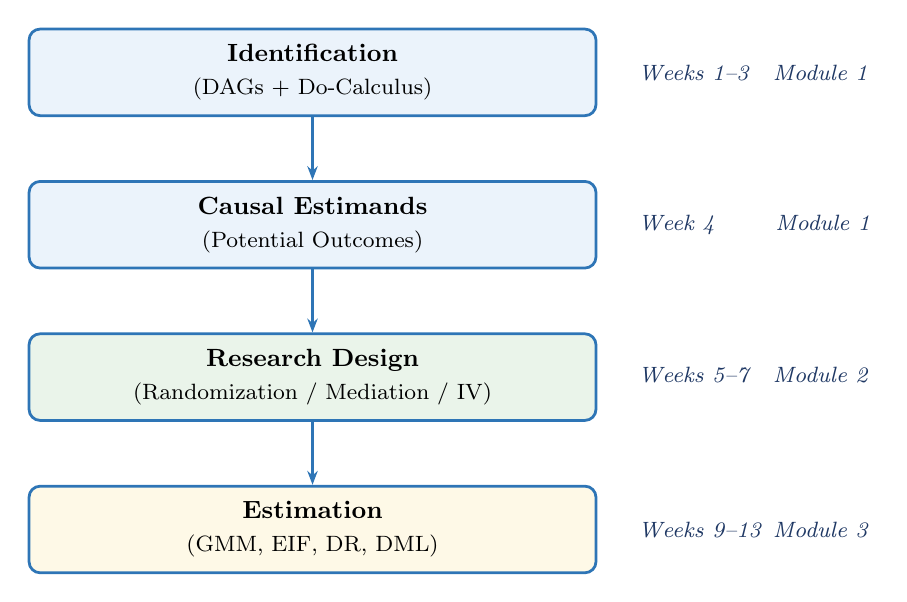
\begin{tikzpicture}[
  node distance = 8mm,
  box/.style = {
    rectangle, rounded corners=4pt,
    minimum width=72mm, minimum height=11mm,
    align=center, font=\small\bfseries,
    draw=midblue, line width=1pt
  },
  label/.style = {
    font=\footnotesize\itshape\color{darkblue},
    anchor=west
  },
  arr/.style = {-{Stealth[length=5pt]}, line width=1pt, color=midblue}
]
  \node[box, fill=mod1]  (id)   {Identification\\[1pt]
    {\normalfont\footnotesize(DAGs + Do-Calculus)}};
  \node[box, fill=mod1,  below=of id]  (po)   {Causal Estimands\\[1pt]
    {\normalfont\footnotesize(Potential Outcomes)}};
  \node[box, fill=mod2,  below=of po]  (rd)   {Research Design\\[1pt]
    {\normalfont\footnotesize(Randomization / Mediation / IV)}};
  \node[box, fill=mod3,  below=of rd]  (est)  {Estimation\\[1pt]
    {\normalfont\footnotesize(GMM, EIF, DR, DML)}};

  \draw[arr] (id)  -- (po);
  \draw[arr] (po)  -- (rd);
  \draw[arr] (rd)  -- (est);

  \node[label] at ([xshift=4mm]id.east)  {Weeks 1--3\quad Module 1};
  \node[label] at ([xshift=4mm]po.east)  {Week 4\qquad\enspace Module 1};
  \node[label] at ([xshift=4mm]rd.east)  {Weeks 5--7\quad Module 2};
  \node[label] at ([xshift=4mm]est.east) {Weeks 9--13\enspace Module 3};
\end{tikzpicture}
\end{center}

\medskip
A central theme is the distinction between the \emph{interventional}
conditional density $f(y \mid x, \mathrm{do}(T{=}t); \theta)$ and the
\emph{observational} conditional density $f(y \mid x, T{=}t)$. In the
Gaussian linear model:

\begin{keybox}
\[
  \underbrace{f\!\bigl(y \mid \mathrm{do}(T{=}t)\bigr)}_{\displaystyle
    = N(\beta t,\;\sigma^2)}
  \;\neq\;
  \underbrace{f\!\bigl(y \mid T{=}t\bigr)}_{\displaystyle
    = N\!\Bigl(\bigl(\beta + \tfrac{\rho\sigma}{\tau}\bigr)t,\;
              \sigma^2(1-\rho^2)\Bigr)}.
\]
\end{keybox}

The do-operator makes this distinction \emph{syntactically enforced},
whereas the potential-outcomes framework leaves it implicit.

The 15-week format at Iowa State provides breathing room that a compressed
version cannot: the dense graphical theory (DAGs and $d$-separation) is
separated from the do-calculus rules into two distinct weeks, potential
outcomes receive their own full week \emph{after} the identification machinery
is in place, and mediation analysis receives a dedicated week before
instrumental variables are introduced.

% ════════════════════════════════════════════════════════════════════════════
\section{Module 1: Foundations (Weeks 1--4)}
% ════════════════════════════════════════════════════════════════════════════

The first module establishes the conceptual and mathematical infrastructure
on which the rest of the course rests. Each of its four weeks is genuinely
self-contained: the first builds physical intuition for the do-operator, the
second develops the graphical language for reading independence claims, the
third translates that language into identification formulas via the three
rules of do-calculus, and the fourth places the potential-outcomes framework
alongside do-calculus so students see where the two traditions agree and
where they diverge.
Module~2 then studies three concrete identification settings ---
randomized experiments, mediation analysis, and instrumental variables ---
that together cover the main strategies for handling direct effects, indirect
effects, and unmeasured confounding.

% ── Week 1 ───────────────────────────────────────────────────────────────────
\subsection{Week 1: The Interventional/Observational Distinction}

This is the conceptual core of the entire course and deserves a full week.
The central question is: \emph{what does it mean to ask ``what would happen
if we set $T = t$?''} The answer is developed through two complementary
representations, with a brief preview of a third.

\begin{itemize}
  \item \textbf{Structural equation model.}
    $Y = f(T, U, \varepsilon)$ and the effect of replacing the equation for
    $T$ with the constant $T = t$ (do-operator as equation surgery).

  \item \textbf{Graphical model.}
    The do-operator as graph surgery --- removing all arrows into $T$ in the
    DAG.

  \item \textbf{Potential outcomes model (preview).}
    $Y(t)$ as a random variable on an extended probability space.
    This third representation is introduced briefly here to complete
    the trinity of causal frameworks; its full development---and its
    precise relationship to the do-calculus---is deferred to Week~4,
    after the identification machinery has been established.
\end{itemize}

The key equation motivating the entire course is derived explicitly:
\begin{keybox}
\[
  f\!\bigl(y \mid x,\, T{=}t\bigr)
  \;=\;
  \int f\!\bigl(y \mid x,\,\mathrm{do}(T{=}t),\, U{=}u\bigr)\;
       p(u \mid x, T{=}t)\; du
  \;\neq\;
  f\!\bigl(y \mid x,\,\mathrm{do}(T{=}t)\bigr).
\]
The gap is exactly the endogeneity bias that causal inference must overcome.
\end{keybox}

The Gaussian linear IV model is introduced as a running example, with
explicit calculations showing the bias term $\rho\sigma/\tau$ separating
the two densities.

\smallskip
\noindent\textit{Reading:} Pearl, Glymour \& Jewell (2016), Ch.~1--4;
Hern\'an \& Robins (2020), Ch.~1--3.

% ── Week 2 ───────────────────────────────────────────────────────────────────
\subsection{Week 2: Directed Acyclic Graphs and \textit{d}-Separation}

In the 15-week format, the graphical theory is given a full week before
the do-calculus rules are introduced. This separation allows students to
become fluent in reading conditional independence from DAGs before they
are asked to manipulate interventional expressions.

\begin{itemize}
  \item \textbf{Directed acyclic graphs.}
    Nodes, directed edges, parents, ancestors, descendants. The acyclicity
    condition and why it is necessary for the Markov factorisation.

  \item \textbf{Global Markov condition.}
    Every variable is independent of its non-descendants given its parents;
    the joint density factorises as
    $p(v_1,\ldots,v_k) = \prod_i p(v_i \mid \mathrm{Pa}(v_i))$.

  \item \textbf{Three path structures.}
    Chain $A \to M \to B$ (blocked by conditioning on $M$);
    fork $A \leftarrow M \rightarrow B$ (blocked by conditioning on $M$);
    collider $A \to C \leftarrow B$ (blocked by default; \emph{opened} by
    conditioning on $C$ or any descendant).

  \item \textbf{\textit{d}-Separation.}
    Formal definition and the Verma--Pearl (1988) theorem: $d$-separation
    implies conditional independence in every distribution Markov with
    respect to the graph.

  \item \textbf{The collider trap.}
    Berkson's bias as an instance of conditioning on a collider. Application
    to the IV DAG: why conditioning on $T$ (the collider in
    $Z \to T \leftarrow U$) opens a back-door path from $Z$ to $Y$.

  \item \textbf{Extended example.}
    Full $d$-separation analysis of the IV DAG
    $\{Z \to T, T \to Y, U \to T, U \to Y\}$ for all interesting
    conditioning sets.
\end{itemize}

\noindent\textit{Reading:} Pearl, Glymour \& Jewell (2016), Ch.~2--3;
Pearl (2000), Ch.~1--2.

% ── Week 3 ───────────────────────────────────────────────────────────────────
\subsection{Week 3: The Do-Calculus and Identification Criteria}

With $d$-separation in hand, students are now ready for the algebraic
machinery that translates graph surgery into identification formulas.

\begin{itemize}
  \item \textbf{Mutilated graphs.}
    $\mathcal{G}_{\overline{X}}$ (delete arrows into $X$) and
    $\mathcal{G}_{\underline{X}}$ (delete arrows out of $X$).

  \item \textbf{Three rules of do-calculus (Pearl, 1995).}
    \begin{itemize}
      \item Rule~1 (insertion/deletion of observations):
        $P(y \mid \mathrm{do}(x), z, w) = P(y \mid \mathrm{do}(x), w)$
        if $(Y \perp\!\!\!\perp Z \mid X,W)_{\mathcal{G}_{\overline{X}}}$.
      \item Rule~2 (action/observation exchange):
        $P(y \mid \mathrm{do}(x),\mathrm{do}(z),w)
         = P(y \mid \mathrm{do}(x),z,w)$
        if $(Y \perp\!\!\!\perp Z \mid X,W)_{\mathcal{G}_{\overline{X}\underline{Z}}}$.
      \item Rule~3 (insertion/deletion of actions):
        $P(y \mid \mathrm{do}(x),\mathrm{do}(z),w)
         = P(y \mid \mathrm{do}(x),w)$
        if $(Y \perp\!\!\!\perp Z \mid X,W)_{\mathcal{G}_{\overline{X}\,\overline{Z(W)}}}$.
    \end{itemize}

  \item \textbf{Back-door criterion.}
    Definition, derivation via Rules~2--3, and the adjustment formula:
    \[
      f\!\bigl(y \mid \mathrm{do}(T{=}t)\bigr)
      = \int f(y \mid t,x)\, p(x)\, dx.
    \]
    Why condition~(1) (no descendant of $T$ in the adjustment set) is
    essential.

  \item \textbf{Front-door criterion.}
    Identification through a mediator $M$ when the confounder is
    unobserved:
    \[
      f\!\bigl(y \mid \mathrm{do}(T{=}t)\bigr)
      = \int P(m \mid t) \int P(y \mid t', m)\, P(t')\, dt'\; dm.
    \]

  \item \textbf{Completeness (Shpitser \& Pearl, 2006).}
    The do-calculus is complete: if $P(y \mid \mathrm{do}(t))$ is not
    identifiable by the three rules, it is genuinely non-identified.
\end{itemize}

\noindent\textit{Reading:} Pearl (2000), Ch.~3--4.

% ── Week 4 ───────────────────────────────────────────────────────────────────
\subsection{Week 4: Potential Outcomes and the Connection to Do-Calculus}

With both the do-calculus and its identification criteria fully established,
Week~4 introduces the Neyman--Rubin potential outcomes framework as the
natural language for defining causal estimands. Students encounter this
framework after the identification machinery of Weeks~1--3 has already
shown how causal quantities can be recovered from observational data.
The framework is powerful for defining estimands precisely but, as
students can now appreciate, silent on the identification problem the
preceding three weeks have solved.

\begin{itemize}
  \item \textbf{Rubin's potential outcomes.}
    $Y(t)$, SUTVA, and the consistency assumption $Y(t) = Y$ when $T = t$.
    Connection to $f(y \mid \mathrm{do}(T{=}t))$ via SUTVA.

  \item \textbf{Ignorability.}
    $(Y(0), Y(1)) \perp\!\!\!\perp T \mid X$ and its relationship to the
    back-door criterion: ignorability is exactly the graphical condition
    that $X$ blocks all back-door paths.

  \item \textbf{Single World Intervention Graphs (SWIGs).}
    Richardson \& Robins (2014): graphical representation of potential
    outcomes that bridges the two frameworks and makes
    cross-world independence assumptions visible.

  \item \textbf{Where the frameworks agree and diverge.}
    Both define causal estimands clearly. The do-calculus enforces the
    interventional/observational distinction syntactically; potential
    outcomes leave it implicit. For likelihood-based inference, the
    do-calculus is indispensable.

  \item \textbf{Module~1 synthesis.}
    The running Gaussian linear IV example is revisited: students can
    now give a complete account of the endogeneity problem in all three
    languages (SEM, DAG, potential outcomes) and understand why the
    do-operator language is the most precise for the likelihood
    construction studied in Week~12.
\end{itemize}

\noindent\textit{Reading:} Richardson \& Robins (2014);
Imbens \& Rubin (2015), Ch.~1--2.

% ════════════════════════════════════════════════════════════════════════════
\section{Module 2: Identification Theory (Weeks 5--8)}
% ════════════════════════════════════════════════════════════════════════════

Module~2 studies three identification strategies in increasing order of
difficulty. Randomization (Week~5) provides the simplest setting in which
$\mathrm{do}(T{=}t)$ is directly observable. Mediation analysis (Week~6)
asks how much of the total effect flows through an intermediate variable,
requiring two-stage identification. Instrumental variables (Week~7) handle
unmeasured confounding via an exogenous shifter. Week~8 is the first midterm
examination.

% ── Week 5 ───────────────────────────────────────────────────────────────────
\subsection{Week 5: Randomization and Its Surrogates}

\begin{itemize}
  \item \textbf{Randomized experiments.}
    Under randomization $\mathrm{do}(T{=}t)$ is directly observed, so
    $f(y \mid \mathrm{do}(T{=}t)) = f(y \mid T{=}t)$.
    Why this equality holds graphically (no arrows into $T$ in the
    experimental design).

  \item \textbf{Propensity score.}
    $e(X) = P(T{=}1 \mid X)$.  Balancing property:
    $Y(t) \perp\!\!\!\perp T \mid e(X)$.
    Justifies back-door adjustment on $e(X)$ alone.
    Estimation via logistic regression and machine learning.

  \item \textbf{Overlap and positivity.}
    The strict overlap condition $0 < e(X) < 1$; practical consequences
    of near-violations and trimming strategies.

  \item \textbf{Limitation.}
    Back-door adjustment requires no unmeasured confounders --- a strong
    and untestable assumption. This motivates the mediation and IV
    strategies of Weeks~6--7.
\end{itemize}

\noindent\textit{Reading:} Hern\'an \& Robins (2020), Ch.~7--9.

% ── Week 6 ───────────────────────────────────────────────────────────────────
\subsection{Week 6: Mediation Analysis}

Mediation analysis decomposes the total causal effect of $T$ on $Y$ into
a component operating \emph{through} an intermediate variable $M$ (the
indirect effect) and a component that bypasses $M$ (the direct effect).
Knowing \emph{how} a treatment works---not just whether it works---is
essential for mechanism-based intervention design and is one of the most
common questions in applied causal inference.

\begin{itemize}
  \item \textbf{The mediation DAG.}
    $T \to M \to Y$, $T \to Y$, with possible unobserved confounders
    of each pathway. Preview of why the second-stage identification
    problem ($M \to Y$) is harder than the first.

  \item \textbf{Controlled Direct Effect (CDE).}
    \[
      \mathrm{CDE}(m)
      = E\!\bigl[Y\bigl(\mathrm{do}(T{=}1, M{=}m)\bigr)\bigr]
      - E\!\bigl[Y\bigl(\mathrm{do}(T{=}0, M{=}m)\bigr)\bigr].
    \]
    Identification via back-door adjustment when no unmeasured $M$--$Y$
    confounding is present; the set $(T, X)$ is a valid adjustment set
    for the $M \to Y$ regression under Assumption~3.

  \item \textbf{Identifying the component pathways.}
    \begin{itemize}
      \item \emph{First stage ($T \to M$):} identified by back-door
        adjustment on $X$ alone; randomisation of $T$ suffices.
      \item \emph{Second stage ($M \to Y$ given $T$):} requires no
        unmeasured $M$--$Y$ confounding conditional on $(T, X)$ ---
        an assumption that randomisation of $T$ does \emph{not}
        guarantee. This is the critical identification challenge in
        mediation analysis.
    \end{itemize}

  \item \textbf{The Baron--Kenny linear mediation model.}
    Three-equation system:
    \begin{align*}
      Y &= \alpha_1 + \tau T + \gamma_1 X + \varepsilon_1, \\
      M &= \alpha_2 + a T + \gamma_2 X + \varepsilon_2, \\
      Y &= \alpha_3 + \tau' T + b M + \gamma_3 X + \varepsilon_3.
    \end{align*}
    Product formula $\tau = \tau' + ab$ (total $=$ direct $+$ indirect);
    algebraic proof via substitution. The Sobel test for $H_0: ab = 0$
    using the delta-method variance
    $\widehat{\mathrm{Var}}(ab) \approx b^2 \hat\sigma_a^2
     + a^2 \hat\sigma_b^2$.

  \item \textbf{Four identification assumptions.}
    (1)~No unmeasured $T$--$Y$ confounding; (2)~no unmeasured $T$--$M$
    confounding; (3)~no unmeasured $M$--$Y$ confounding given $T$
    [critical: never guaranteed by randomisation]; (4)~no $T \times M$
    interaction on $Y$.  Each assumption is interpreted graphically.

  \item \textbf{Front-door criterion as full mediation.}
    When there is no direct $T \to Y$ edge and the front-door graph holds,
    Assumption~3 is automatically satisfied (no back-door path from $M$
    to $Y$ survives), and the front-door formula provides complete
    identification without randomising $T$.

  \item \textbf{Natural effects (preview).}
    Natural Direct Effect
    $\mathrm{NDE} = E[Y(1, M(0)) - Y(0, M(0))]$ and Natural Indirect Effect
    $\mathrm{NIE} = E[Y(1, M(1)) - Y(1, M(0))]$;
    cross-world independence and why they require stronger assumptions
    than the CDE. In the linear Baron--Kenny model without interaction,
    NDE $= \tau'$ and NIE $= ab$, so the product formula recovers
    natural effects automatically.
\end{itemize}

\noindent\textit{Reading:} Baron \& Kenny (1986);
Pearl (2000), Ch.~4 (front-door); VanderWeele (2015), Ch.~2--3.

% ── Week 7 ───────────────────────────────────────────────────────────────────
\subsection{Week 7: Instrumental Variables --- Identification}

Instrumental variables provide identification of causal effects when
unmeasured confounding makes back-door adjustment infeasible.  This week
develops the IV assumptions in all three languages used in the literature,
derives the key identification results, and previews the likelihood problem
that will be studied in Module~3.

\subsubsection*{The Three IV Assumptions}

The IV assumptions take different forms depending on the framework.
Students must be able to move fluently between these representations,
since different papers use different conventions.

\begin{center}
\renewcommand{\arraystretch}{1.6}
\small
\begin{tabular}{@{}p{2.2cm} p{4.0cm} p{4.0cm} p{4.0cm}@{}}
  \toprule
  \textbf{Assumption}
    & \textbf{Potential outcomes}
    & \textbf{Structural / econometric}
    & \textbf{Do-calculus / graphical} \\
  \midrule
  Relevance
    & $Z \not\!\perp\!\!\!\perp T$
    & $\mathrm{Cov}(Z, T) \neq 0$
    & No $d$-separation of $Z$ and $T$ in $\mathcal{G}$ \\
  Exogeneity
    & $Z \perp\!\!\!\perp \bigl(Y(0), Y(1), T(0), T(1)\bigr) \mid X$
      (as-good-as-random assignment of $Z$)
    & $E[\varepsilon \mid Z, X] = 0$
    & $Z \perp\!\!\!\perp U \mid X$
      (no back-door path from $Z$ to $Y$ via $U$) \\
  Exclusion
    & $Y_i(t, z) = Y_i(t, z')$ for all $z, z'$
      (instrument affects $Y$ only through $T$)
    & $Z$ excluded from the structural equation for $Y$;
      $\mathrm{Cov}(Z, \varepsilon) = 0$
    & $f(y \mid x, \mathrm{do}(T{=}t), z)
       = f(y \mid x, \mathrm{do}(T{=}t))$
       (Rule~1 in $\mathcal{G}_{\overline{T}}$) \\
  \bottomrule
\end{tabular}
\end{center}

\medskip
The do-calculus column is the course's preferred framing because it is
syntactically unambiguous: the exclusion restriction is visibly a statement
about the interventional density, not the observational one.  The potential
outcomes column is the language of Angrist, Imbens \& Rubin (1996) and most
of the biostatistics literature.  The structural column is standard in
econometrics.

\subsubsection*{The Wald Estimand}

Under the three IV assumptions, in the linear structural model
$Y = \alpha + \beta T + \varepsilon$, $T = \pi Z + \delta$,
$\mathrm{Cov}(\varepsilon, \delta) = \rho\sigma\tau \neq 0$:

\begin{keybox}
\[
  \beta
  \;=\; E\!\bigl[Y \mid \mathrm{do}(T{=}t{+}1)\bigr]
        - E\!\bigl[Y \mid \mathrm{do}(T{=}t)\bigr]
  \;=\; \frac{\mathrm{Cov}(Y, Z)}{\mathrm{Cov}(T, Z)}
  \;=\; \frac{E[Y \mid Z{=}1] - E[Y \mid Z{=}0]}
             {E[T \mid Z{=}1] - E[T \mid Z{=}0]}.
\]
The right-hand side involves only observational quantities and is the
\textbf{Wald estimand}.
\end{keybox}

\noindent\textit{Derivation via do-calculus.}  In the mutilated graph
$\mathcal{G}_{\overline{T}}$, exogeneity gives $Z \indep U \mid X$ and
the exclusion restriction (Rule~1) removes $Z$ from the density of $Y$
given $\mathrm{do}(T{=}t)$.  Relevance ensures the denominator is
non-zero.  The ratio then follows from the linear projection of $Y$ onto
$Z$, using $E[\varepsilon \mid Z] = 0$.

\subsubsection*{Two-Stage Least Squares}

In the multi-instrument or covariate-adjusted setting, 2SLS generalises
the Wald estimand:
\begin{enumerate}
  \item \textbf{First stage.}  Regress $T$ on $(Z, X)$; obtain fitted
    values $\hat{T} = \hat{E}[T \mid Z, X]$.
  \item \textbf{Second stage.}  Regress $Y$ on $(\hat{T}, X)$; the
    coefficient on $\hat{T}$ is the 2SLS estimator $\hat\beta_{\mathrm{2SLS}}$.
\end{enumerate}
Under the IV assumptions, $\hat\beta_{\mathrm{2SLS}} \xrightarrow{p} \beta$
and $\sqrt{n}(\hat\beta_{\mathrm{2SLS}} - \beta) \xrightarrow{d} N(0, V)$
with the standard sandwich variance.

\subsubsection*{The LATE Theorem}

In the binary-instrument, binary-treatment setting ($Z, T \in \{0,1\}$),
IV does not generally identify the average treatment effect (ATE) unless
the treatment effect is homogeneous.  Under an additional
\textbf{monotonicity} assumption --- $T_i(1) \geq T_i(0)$ for all $i$
(no defiers) --- Angrist \& Imbens (1994) show:

\begin{keybox}
\[
  \frac{E[Y \mid Z{=}1] - E[Y \mid Z{=}0]}
       {E[T \mid Z{=}1] - E[T \mid Z{=}0]}
  \;=\; E\!\bigl[Y(1) - Y(0) \;\big|\; T_i(1) > T_i(0)\bigr]
  \;\equiv\; \mathrm{LATE}.
\]
\end{keybox}

The Wald estimand identifies the \textbf{Local Average Treatment Effect}:
the average causal effect for \emph{compliers} --- units whose treatment
status is changed by the instrument.  This is generally different from the
ATE or the ATT.  Key implications:
\begin{itemize}
  \item LATE is the identified estimand under heterogeneous treatment effects;
    the ATE requires additional homogeneity assumptions.
  \item Different instruments (with different complier populations) identify
    different LATEs --- an important point for interpreting IV estimates
    across studies.
  \item In the homogeneous-effects linear model, LATE $= \beta =$ ATE, so
    the distinction collapses.
\end{itemize}

\noindent\textit{Reading:} Angrist \& Imbens (1994);
Angrist, Imbens \& Rubin (1996);
Hern\'an \& Robins (2020), Ch.~16.

% ────────────────────────────────────────────────────────────────────────────
\subsection*{Week 8: Midterm Examination 1}
\addcontentsline{toc}{subsection}{Week 8: Midterm Examination 1}
% ────────────────────────────────────────────────────────────────────────────

\begin{exambox}
\noindent\textbf{\color{darkblue}Midterm Examination 1 --- Week 8.}
The first midterm covers Modules~1--2 (Weeks~1--7).  It is a closed-book,
in-class examination of 80 minutes.  The examination consists of three
parts:

\begin{enumerate}
  \item \textbf{Graphical reasoning (35\%).}
    Given a DAG, determine $d$-separation relationships, identify valid
    adjustment sets, and classify a proposed estimator as back-door,
    front-door, or neither.

  \item \textbf{Do-calculus derivations (35\%).}
    Apply the three rules to derive identification formulas from first
    principles; prove or disprove specific identification claims; derive
    the CDE identification formula or the IV Wald estimand from stated
    assumptions.

  \item \textbf{Short-answer conceptual questions (30\%).}
    Explain the critical assumption in mediation analysis (no unmeasured
    $M$--$Y$ confounding), the exclusion restriction as a do-calculus
    statement, or the distinction between NDE/NIE and CDE.
\end{enumerate}

\noindent\textbf{No new content is introduced this week.}
A review session in the lecture period before the examination summarises
the key results of Modules~1--2.
\end{exambox}

% ════════════════════════════════════════════════════════════════════════════
\section{Module 3: Estimation Theory (Weeks 9--13)}
% ════════════════════════════════════════════════════════════════════════════

This module is where expertise in survey sampling, calibration, and
semiparametric theory becomes directly relevant.  The GEC framework,
Bregman projections, and SREG estimators developed in the instructor's
research programme provide a thread of novel methodology alongside the
classical material.

% ── Week 9 ───────────────────────────────────────────────────────────────────
\subsection{Week 9: From Identification to Estimation ---
  GMM and the EIF}

Once identification is established, the causal effect is a functional
of the observed data distribution: $\psi = \Psi(P)$.  The central
question of this week is: \emph{how do we go from an identified moment
condition to an estimator, and which moment function should we use?}
GMM is the classical answer; the efficient influence function (EIF) is
the semiparametric answer.  They are two sides of the same coin.

\subsubsection*{Part I: GMM as the Bridge from Identification to
  Estimation}

Both the back-door and the IV identification strategies produce a
\textbf{moment condition} of the form
\[
  E\!\bigl[\psi(Y, T, X, Z;\theta_0)\bigr] = 0,
\]
where $\psi$ is called the \emph{estimating function} or \emph{moment
function}.  The identification step guarantees this holds at the true
$\theta_0$; the estimation step solves the sample analogue.

\begin{itemize}
  \item \textbf{Examples of moment conditions from identification.}
    \begin{itemize}
      \item \emph{Back-door (exogenous $T$):}
        $\psi_i = \partial_\theta \log f(y_i \mid t_i, x_i;\theta)$
        (the score).  This is the MLE first-order condition.
      \item \emph{IV moment condition:}
        $\psi_i = (y_i - \mu(t_i, x_i;\theta))\cdot z_i$.
        Identification gives $E[\varepsilon \cdot Z] = 0$ at $\theta_0$;
        GMM solves the sample version.
      \item \emph{Overidentified IV (multiple instruments):}
        $\psi_i \in \mathbb{R}^q$ with $q > \dim(\theta)$.
        GMM minimises $\bar\psi(\theta)^\top W \bar\psi(\theta)$ over
        a weight matrix $W$.
    \end{itemize}

  \item \textbf{GMM estimator (Hansen, 1982).}
    \[
      \hat\theta_{\mathrm{GMM}}
      = \arg\min_\theta\;
        \bar\psi(\theta)^\top \hat W\, \bar\psi(\theta),
        \qquad
        \bar\psi(\theta) = \frac{1}{n}\sum_{i=1}^n \psi_i(\theta).
    \]
    Under standard regularity conditions:
    \[
      \sqrt{n}(\hat\theta_{\mathrm{GMM}} - \theta_0)
      \xrightarrow{d} N\!\bigl(0,\; (G^\top W G)^{-1}
        G^\top W \Sigma W G\, (G^\top W G)^{-1}\bigr),
    \]
    where $G = E[\partial_\theta \psi(\theta_0)]$ and
    $\Sigma = \mathrm{Var}[\psi(\theta_0)]$.
    This is the \textbf{sandwich variance} --- it appears whenever the
    moment function is not the score of a correctly specified model.

  \item \textbf{Optimal GMM.}
    The variance-minimising weight matrix is $W^* = \Sigma^{-1}$, giving
    the \emph{efficient GMM} variance $(G^\top \Sigma^{-1} G)^{-1}$.
    In the just-identified case ($q = \dim(\theta)$), $W$ cancels and
    all weight matrices give the same estimator.  2SLS is efficient GMM
    in the linear IV model with homoskedastic errors.

  \item \textbf{Deriving the IV moment condition from the do-calculus
    assumptions.}
    This is the key connection that is often left implicit in the
    literature.  Start from the structural model
    $Y = \mu(T, X;\theta) + \varepsilon$ and the three IV assumptions
    as stated in Week~7.

    \begin{enumerate}
      \item \emph{Exogeneity} ($Z \indep U \mid X$) says that the
        instrument is independent of the unobserved confounder.
        Since $\varepsilon = Y - \mu(T,X;\theta_0)$ is a function of
        $U$ (through the structural equation), exogeneity implies
        \[
          E[\varepsilon \mid X, Z] = E[\varepsilon \mid X].
        \]

      \item \emph{Exclusion restriction}
        ($f(y \mid x, \mathrm{do}(T{=}t), z)
         = f(y \mid x, \mathrm{do}(T{=}t))$)
        says $Z$ has no direct effect on $Y$ once $T$ is set by
        intervention.  In the structural equation, $Z$ enters only
        through $T$, so $\varepsilon$ is mean-independent of $Z$
        given $X$:
        \[
          E[\varepsilon \mid X, Z] = E[\varepsilon \mid X].
        \]
        Together with the \emph{normalisation}
        $E[\varepsilon \mid X] = 0$ (which is without loss of
        generality by absorbing any non-zero mean into
        $\mu(T,X;\theta)$), we obtain
        \[
          E[\varepsilon \mid X, Z] = 0.
        \]

      \item Taking unconditional expectations of
        $\varepsilon \cdot (Z - E[Z \mid X])$ gives the
        \textbf{IV moment condition}:
        \[
          \boxed{E\!\bigl[\varepsilon(T, X;\theta_0) \cdot Z\bigr]
          = E\!\bigl[(Y - \mu(T, X;\theta_0))\cdot Z\bigr] = 0.}
        \]
        (After partialling out $X$; the centred version
        $(Z - E[Z\mid X])$ is used when $X$ is present.)
    \end{enumerate}

    This derivation makes the chain explicit:
    \emph{do-calculus exogeneity and exclusion}
    $\Rightarrow$ $E[\varepsilon \mid X, Z] = 0$
    $\Rightarrow$ IV moment condition
    $\Rightarrow$ GMM estimating equation.
    No model for $U$ and no full observed-data likelihood are required
    at any step --- which is precisely why GMM is the natural
    estimation framework in econometrics whenever identification rests
    on an instrument.
\end{itemize}

\subsubsection*{Part II: The EIF as the Optimal Moment Function}

GMM can use \emph{any} valid moment function $\psi$ satisfying
$E[\psi(\theta_0)] = 0$.  Semiparametric efficiency theory asks:
which choice of $\psi$ minimises the asymptotic variance?  The answer
is the \textbf{efficient influence function} (EIF).

\begin{itemize}
  \item \textbf{Asymptotically linear estimators.}
    An estimator $\hat\psi$ is asymptotically linear with influence
    function $\varphi$ if
    \[
      \sqrt{n}(\hat\psi - \psi_0)
      = \frac{1}{\sqrt{n}}\sum_{i=1}^n \varphi(O_i) + o_p(1),
      \qquad E_0[\varphi] = 0.
    \]
    The asymptotic variance is $E_0[\varphi^2]$.  GMM with moment
    function $\psi$ is asymptotically linear with
    $\varphi = -(G^\top W G)^{-1} G^\top W \psi$.

  \item \textbf{Semiparametric efficiency bound (Bickel et al., 1998).}
    Among all regular asymptotically linear estimators:
    \[
      \mathrm{Var}(\hat\psi) \geq E_0\!\bigl[\varphi^*(O)^2\bigr],
    \]
    where $\varphi^*$ is the \textbf{EIF} --- the unique influence
    function that achieves this lower bound.

  \item \textbf{EIF for the ATE under back-door identification.}
    \[
      \varphi^*(O)
      = \mu(1,X) - \mu(0,X)
        + \frac{T\bigl(Y - \mu(1,X)\bigr)}{e(X)}
        - \frac{(1-T)\bigl(Y - \mu(0,X)\bigr)}{1 - e(X)}
        - \psi_0.
    \]
    A GMM estimator using $\varphi^*$ as its moment function achieves
    the efficiency bound; this is exactly the AIPW estimator of
    Week~10.

  \item \textbf{The unifying connection.}
    In a correctly specified \emph{parametric} model, the EIF equals
    the score $\partial_\theta \log f(O;\theta_0)$, and GMM with the
    score is MLE.  The semiparametric efficiency bound therefore
    generalises the Cram\'er--Rao bound to the setting where the
    full data-generating process is only partially specified.

  \item \textbf{Connection to GEC.}
    The EIF is the gradient of the functional $\Psi(P)$ in the Hilbert
    space of mean-zero square-integrable functions.  The generalised
    entropy calibration (GEC) estimator achieves the semiparametric
    bound by solving a constrained entropy problem whose first-order
    conditions reproduce the EIF estimating equation --- connecting
    calibration weighting directly to optimal GMM.

  \item \textbf{Influence function arithmetic.}
    Linearity, the product rule, and the delta method for smooth
    functionals of $P$; used to derive EIFs for ATE, ATT, and
    dose-response curves in subsequent weeks.
\end{itemize}

\begin{keybox}
\noindent\textbf{The GMM--EIF hierarchy.}
Any valid moment condition $\Rightarrow$ consistent GMM estimator with
sandwich variance.  The EIF moment condition $\Rightarrow$ efficient
GMM estimator achieving the semiparametric bound.  MLE in a correctly
specified model $\Rightarrow$ EIF = score $\Rightarrow$ Cram\'er--Rao
bound.  Each step adds assumptions and gains efficiency.
\end{keybox}

\noindent\textit{Reading:} Hansen (1982); Tsiatis (2006);
Bickel et al.\ (1998); Newey \& McFadden (1994).

% ── Week 10 ──────────────────────────────────────────────────────────────────
\subsection{Week 10: IPW, Outcome Regression, and Doubly Robust Estimation}

\begin{itemize}
  \item \textbf{IPW estimator.}
    \[
      \hat\tau_{\mathrm{IPW}} = \frac{1}{n}\sum_{i=1}^n \left[
        \frac{T_i Y_i}{\hat e(X_i)} - \frac{(1-T_i)Y_i}{1-\hat e(X_i)}
      \right].
    \]
    Consistency and $\sqrt{n}$-rate under correct propensity model;
    efficiency loss relative to EIF.

  \item \textbf{Outcome regression.}
    \[
      \hat\tau_{\mathrm{OR}} = \frac{1}{n}\sum_{i=1}^n
        \bigl[\hat\mu(1, X_i) - \hat\mu(0, X_i)\bigr].
    \]

  \item \textbf{AIPW / doubly robust estimator.}
    \[
      \hat\tau_{\mathrm{DR}} = \hat\tau_{\mathrm{OR}}
        + \frac{1}{n}\sum_{i=1}^n
          \frac{T_i - \hat e(X_i)}{\hat e(X_i)(1-\hat e(X_i))}
          \bigl(Y_i - \hat\mu(T_i, X_i)\bigr).
    \]
    Doubly robust consistency, efficiency, and the relation to the EIF.

  \item \textbf{Connection to calibration weighting.}
    The GEC framework as a generalisation of IPW incorporating
    covariate balance constraints: the calibration weights solve
    $\min_w D_\phi(w \| q)$ subject to $\sum_i w_i h(X_i) = \bar h$,
    reproducing IPW at the entropic divergence.
\end{itemize}

\noindent\textit{Reading:} Bang \& Robins (2005);
Hern\'an \& Robins (2020), Ch.~13.

% ── Week 11 ──────────────────────────────────────────────────────────────────
\subsection{Week 11: Doubly Robust Estimation in the IV Setting}

\begin{itemize}
  \item \textbf{DR IV estimating equation.}
    \[
      U_{\mathrm{DR}}(\theta) = \frac{1}{n}\sum_{i=1}^n
        \Psi(Y_i, T_i, X_i, Z_i;\theta, \hat\phi, \hat\mu) = 0,
    \]
    where $\Psi$ uses the ratio $T/g(X,Z;\hat\phi)$ as the ``IPW
    weight'' for the instrument.

  \item \textbf{Two distinct robustness mechanisms.}
    \begin{itemize}
      \item \emph{Case~(i), correct $f$:} Fisher score identity forces
        $\mu_0 \equiv 0$; exclusion restriction ensures uniform validity
        over $Z$.
      \item \emph{Case~(ii), correct $g$:} Consistency follows from the
        definition of $\mu_0$ alone, for any $f$.
    \end{itemize}

  \item \textbf{Neyman orthogonality.}
    \[
      E_0\!\left[\frac{\partial \log f_m}{\partial\theta} \cdot
                \frac{\partial \log g}{\partial\phi^\top}\right] = 0
      \quad\text{at }(\theta_0,\phi_0).
    \]
    First-stage estimation error does not inflate the asymptotic
    variance of $\hat\theta$ at the $\sqrt{n}$ rate.
\end{itemize}

\noindent\textit{Reading:} Tchetgen Tchetgen (2017);
Chernozhukov et al.\ (2018).

% ── Week 12 ──────────────────────────────────────────────────────────────────
\subsection{Week 12: Double Machine Learning and Cross-Fitting}

\begin{itemize}
  \item \textbf{Double machine learning (DML).}
    Use ML to estimate nuisance functions $e_0$ and $\mu_0$ at a
    potentially slow rate, while retaining $\sqrt{n}$-consistency for
    $\theta_0$ via Neyman orthogonality.

  \item \textbf{Product bias condition.}
    \[
      \|\hat e - e_0\| \cdot \|\hat\mu - \mu_0\| = o_p(n^{-1/2})
    \]
    is sufficient for $\sqrt{n}$-estimation even when each factor
    converges at $o_p(n^{-1/4})$.

  \item \textbf{Cross-fitting in detail.}
    $K$-fold sample splitting; removing overfitting bias of order
    $(\hat e - e_0)(\hat\mu - \mu_0)$; the role of cross-fitting in
    ensuring oracle rates for the causal parameter.
\end{itemize}

\noindent\textit{Reading:} Chernozhukov et al.\ (2018).

% ── Week 13 ──────────────────────────────────────────────────────────────────
\subsection{Week 13: Generalised Empirical Likelihood, Regularisation,
  and Calibration}

This week has two connected themes.  The first revisits the GMM moment
condition of Week~9 and asks: is there a more efficient way to solve it
than standard GMM?  The answer is the \textbf{generalised empirical
likelihood} (GEL) family of Newey \& Smith (2004), which achieves higher-order
efficiency and includes the GEC calibration framework as a special case.
The second theme extends these ideas to the high-dimensional setting
where $\dim(X) \gg n$.

\begin{itemize}
  \item \textbf{The GEL problem (Newey \& Smith, 2004).}
    Standard GMM minimises a quadratic form in the sample moments.
    GEL replaces this with a \emph{divergence} between an implied
    probability distribution and the empirical distribution.  Given
    moment conditions $E[\psi(O;\theta)] = 0$, the GEL estimator solves
    \[
      \hat\theta_{\mathrm{GEL}}
      = \arg\min_\theta \max_\lambda
        \sum_{i=1}^n h\!\bigl(\lambda^\top \psi_i(\theta)\bigr),
    \]
    where $h(\cdot)$ is a concave function whose choice determines
    the member of the GEL family.  The implied weights on observations
    are $\hat w_i \propto -h'\!\bigl(\hat\lambda^\top \psi_i(\hat\theta)\bigr)$.

  \item \textbf{The GEL family and Bregman divergences.}
    \begin{center}
    \renewcommand{\arraystretch}{1.4}
    \small
    \begin{tabular}{@{}lll@{}}
      \toprule
      \textbf{Method} & \textbf{$h(v)$} & \textbf{Divergence} \\
      \midrule
      Empirical likelihood (EL)
        & $\log(1 - v)$ & KL divergence $D_{\mathrm{KL}}(P \| Q)$ \\
      Exponential tilting (ET)
        & $-e^v$ & KL divergence $D_{\mathrm{KL}}(Q \| P)$ \\
      Continuous updating GMM
        & $-\tfrac{1}{2}(1-v)^2$ & $\chi^2$ divergence \\
      GEC (Kwon, Kim, and Qiu 2025)
        & General $h$ & General Bregman divergence $D_\phi$ \\
      \bottomrule
    \end{tabular}
    \end{center}

  \item \textbf{Higher-order efficiency of GEL.}
    All GEL estimators share the same first-order asymptotic distribution
    as efficient GMM but GEL eliminates one source of higher-order bias
    (the ``estimation bias''), making GEL preferable in small samples or
    with many moment conditions.

  \item \textbf{Connection to the EIF.}
    When $\psi = \varphi^*$ (the EIF), the GEL estimator is doubly robust
    and achieves the semiparametric efficiency bound --- unifying the GEL
    and EIF perspectives of Week~9.

  \item \textbf{Regularised calibration weights.}
    The GEC framework extended to high dimensions: calibration weights
    solve
    \[
      \min_w\; D_\phi(w \| q)
      \quad\text{subject to}\quad
      \bigl\|A^\top(w - q)\bigr\|_* \leq \lambda,
    \]
    where $A$ is the $n \times p$ covariate matrix and $\|\cdot\|_*$
    is the dual norm.  The H\"older-conjugate penalty structure and
    its connection to the design-optimal estimator; debiased LASSO
    (van de Geer et al., 2014) as a special case.

  \item \textbf{Distributionally robust calibration (DRC).}
    Extend the GEC balance constraint to a Bregman divergence
    ball $D_\phi(Q \| P) \leq \rho$.  The budget parameter $\rho$
    controls the robustness--efficiency trade-off; the minimum feasible
    $\rho$ ($\rho_{\min}$) marks the boundary between feasible and
    infeasible regimes.
\end{itemize}

\begin{keybox}
\noindent\textbf{The GMM -- GEL -- GEC hierarchy.}
Standard GMM: minimise a quadratic in sample moments; sandwich variance;
consistent but not higher-order efficient.
GEL (Newey \& Smith, 2004): minimise a divergence between implied and
empirical weights; same first-order distribution as efficient GMM;
eliminates one second-order bias term.
GEC (Kwon, Kim, and Qiu, 2025): GEL with a general Bregman divergence and
covariate balance constraints; connects to calibration weighting,
IPW, and the EIF estimating equation.
\end{keybox}

\noindent\textit{Reading:} Newey \& Smith (2004);
Kwon, Kim, and Qiu (2025);
van de Geer et al.\ (2014).

% ── Take-Home Midterm 2 ──────────────────────────────────────────────────────
\subsection*{Take-Home Midterm Examination 2
  (distributed end of Week~13, due end of Week~14)}
\addcontentsline{toc}{subsection}{Take-Home Midterm Examination 2
  (Weeks 13--14)}

\begin{exambox}
\noindent\textbf{\color{darkblue}Take-Home Midterm Examination 2.}
Distributed at the end of Week~13; solutions submitted by the end of
Week~14.  The examination covers Module~3 (Weeks~9--13).  Students
work individually; all written sources are permitted but collaboration
is not.  The examination consists of three parts:

\begin{enumerate}
  \item \textbf{GMM and semiparametric efficiency (35\%).}
    Derive the IV moment condition from a stated set of do-calculus
    assumptions; compute the EIF for a given causal functional;
    verify whether a proposed estimator achieves the semiparametric
    efficiency bound.

  \item \textbf{Doubly robust and DML estimation (35\%).}
    Construct and analyse a doubly robust estimator for a specified
    causal parameter; verify Neyman orthogonality; state the product
    bias condition and explain the role of cross-fitting.

  \item \textbf{Regularised calibration (30\%).}
    Formulate a high-dimensional calibration problem as a constrained
    optimisation; derive the first-order conditions and interpret them
    as a moment condition; explain the robustness--efficiency trade-off
    in the DRC framework.
\end{enumerate}

\noindent\textbf{The take-home format} allows for more substantial
derivations and applied problems than an in-class examination.
Students manage the midterm during Weeks~13--14 alongside regular
coursework and final project preparation.
\end{exambox}

% ────────────────────────────────────────────────────────────────────────────
\subsection*{Week 15: Final Presentations}
\addcontentsline{toc}{subsection}{Week 15: Final Presentations}
% ────────────────────────────────────────────────────────────────────────────

\begin{presentbox}
\noindent\textbf{\color{darkblue}Final Presentations --- Week 15.}
Each student (or team of two) presents their final project in a 15-minute
talk (12 minutes + 3 minutes for questions).  Presentations are scheduled
across the Week~15 lecture periods.

\medskip
\noindent\textbf{Presentation requirements:}
\begin{itemize}
  \item Clearly state the causal question and the identification strategy
    (do-calculus language required).
  \item Describe the estimation approach and explain why it achieves the
    semiparametric efficiency bound (or why it does not).
  \item Present simulation or empirical results, including honest
    uncertainty quantification.
  \item Identify one open problem or limitation of your approach.
\end{itemize}

\noindent\textbf{Evaluation criteria (equally weighted):}
identification rigour, estimation soundness, clarity of presentation,
and quality of the written report (submitted one week before
presentations).
\end{presentbox}

% ════════════════════════════════════════════════════════════════════════════
\section{Weekly Schedule at a Glance}
% ════════════════════════════════════════════════════════════════════════════

\begingroup
\small
\setlength{\tabcolsep}{5pt}
\renewcommand{\arraystretch}{1.35}

\begin{longtable}{C{0.6cm} L{1.5cm} L{5.5cm} L{5.8cm}}
  \toprule
  \rowcolor{darkblue}
  \color{white}\textbf{Wk} &
  \color{white}\textbf{Module} &
  \color{white}\textbf{Topic} &
  \color{white}\textbf{Key Readings} \\
  \midrule
  \endfirsthead
  \toprule
  \rowcolor{darkblue}
  \color{white}\textbf{Wk} &
  \color{white}\textbf{Module} &
  \color{white}\textbf{Topic} &
  \color{white}\textbf{Key Readings} \\
  \midrule
  \endhead
  \bottomrule
  \endfoot

  % Module 1
  \rowcolor{mod1}
  1 & Module 1 & The Interventional/Observational Distinction
    & \textit{Pearl et al.\ (2016) Ch.~1--4;
              Hern\'an \& Robins (2020) Ch.~1--3} \\
  \rowcolor{mod1}
  2 & Module 1 & DAGs and $d$-Separation
    & \textit{Pearl et al.\ (2016) Ch.~2--3;
              Pearl (2000) Ch.~1--2} \\
  \rowcolor{mod1}
  3 & Module 1 & The Do-Calculus and Identification Criteria
    & \textit{Pearl (2000) Ch.~3--4} \\
  \rowcolor{mod1}
  4 & Module 1 & Potential Outcomes and Connection to Do-Calculus
    & \textit{Richardson \& Robins (2014);
              Imbens \& Rubin (2015) Ch.~1--2} \\
  \midrule

  % Module 2
  \rowcolor{mod2}
  5 & Module 2 & Randomization and Its Surrogates
    & \textit{Hern\'an \& Robins (2020) Ch.~7--9} \\
  \rowcolor{mod2}
  6 & Module 2 & Mediation Analysis
    & \textit{Baron \& Kenny (1986);
              VanderWeele (2015) Ch.~2--3} \\
  \rowcolor{mod2}
  7 & Module 2 & Instrumental Variables --- Identification
    & \textit{Angrist \& Imbens (1994); Angrist et al.\ (1996);
              Hern\'an \& Robins (2020) Ch.~16} \\
  \midrule

  % Midterm 1
  \rowcolor{examrow}
  8 & \textit{Exam} & \textbf{Midterm Examination 1}
    & \textit{Covers Modules 1--2 (Weeks 1--7)} \\
  \midrule

  % Module 3
  \rowcolor{mod3}
  9 & Module 3 & From Identification to Estimation --- GMM and the EIF
    & \textit{Hansen (1982); Tsiatis (2006); Newey \& McFadden (1994)} \\
  \rowcolor{mod3}
  10 & Module 3 & IPW, Outcome Regression, Doubly Robust Estimation
    & \textit{Bang \& Robins (2005);
              Hern\'an \& Robins (2020) Ch.~13} \\
  \rowcolor{mod3}
  11 & Module 3 & Doubly Robust Estimation in the IV Setting
    & \textit{Tchetgen Tchetgen (2017);
              Chernozhukov et al.\ (2018)} \\
  \rowcolor{mod3}
  12 & Module 3 & Double Machine Learning and Cross-Fitting
    & \textit{Chernozhukov et al.\ (2018)} \\
  \rowcolor{mod3}
  13 & Module 3 & GEL, Regularisation, and Calibration
    & \textit{Newey \& Smith (2004); Kwon, Kim \& Qiu (2025);
              van de Geer et al.\ (2014)} \\
  \midrule

  % Take-home midterm
  \rowcolor{examrow}
  13--14 & \textit{Exam} & \textbf{Take-Home Midterm 2}
    (distributed end of Wk~13, due end of Wk~14)
    & \textit{Covers Module~3 (Weeks 9--13)} \\
  \midrule

  % Presentations
  \rowcolor{presentrow}
  15 & \textit{Pres.} & \textbf{Final Student Presentations}
    & \textit{Written reports due one week prior} \\
  \bottomrule
\end{longtable}
\endgroup

% ════════════════════════════════════════════════════════════════════════════
\section{Assessment}
\label{sec:assessment}
% ════════════════════════════════════════════════════════════════════════════

\begingroup
\small
\setlength{\tabcolsep}{6pt}
\renewcommand{\arraystretch}{1.5}

\begin{tabularx}{\linewidth}{L{3.4cm} C{1.2cm} X}
  \toprule
  \rowcolor{darkblue}
  \color{white}\textbf{Component} &
  \color{white}\textbf{Weight} &
  \color{white}\textbf{Description} \\
  \midrule
  \rowcolor{altrow}
  Problem Sets (3 total) & 25\% &
    One per module (due end of Weeks~4, 7, and 13);
    each requires both identification (do-calculus) and
    estimation components \\
  Midterm Exam 1 (Week 8) & 25\% &
    Closed-book, in-class, 80 minutes;
    covers Modules~1--2 (graphical reasoning,
    do-calculus derivations, mediation and IV identification,
    short conceptual questions) \\
  Midterm Exam 2 (Take-home, Weeks 13--14) & 25\% &
    Take-home; distributed end of Week~13, due end of Week~14;
    covers Module~3 (Weeks~9--13); all written sources permitted,
    no collaboration; includes derivation, applied, and
    regularisation problems \\
  \rowcolor{altrow}
  Final Project \& Presentation & 25\% &
    Written report due one week before presentations;
    in-class presentation in Week~15;
    must develop a new causal inference tool grounded in
    do-calculus identification and semiparametric estimation \\
  \bottomrule
\end{tabularx}
\endgroup

\medskip
\noindent\textbf{Problem set schedule.}
\begin{itemize}
  \item Problem Set 1 (Module 1): due end of Week~4.
    Topics: $d$-separation, do-calculus derivations, back-door and
    front-door identification, potential outcomes and SWIGs.
  \item Problem Set 2 (Module 2): due end of Week~7.
    Topics: propensity score and randomization, mediation identification
    and Baron--Kenny model, IV assumptions and Wald estimand.
  \item Problem Set 3 (Module 3): due end of Week~13.
    Topics: EIF derivation, doubly robust estimation, DML product
    bias condition, regularised calibration weights.
\end{itemize}

% ════════════════════════════════════════════════════════════════════════════
\section{Recommended Core Texts}
% ════════════════════════════════════════════════════════════════════════════

\begingroup
\small
\setlength{\tabcolsep}{6pt}
\renewcommand{\arraystretch}{1.4}

\begin{tabularx}{\linewidth}{L{5.2cm} X}
  \toprule
  \rowcolor{darkblue}
  \color{white}\textbf{Text} &
  \color{white}\textbf{Role in Course} \\
  \midrule
  \rowcolor{altrow}
  \textit{Pearl, Glymour \& Jewell (2016)}
    & Weeks 1--3: do-calculus foundations; primary entry point \\
  \textit{Hern\'an \& Robins (2020)}
    & Weeks 4--11: bridge from identification to statistical
      estimation; freely available online \\
  \rowcolor{altrow}
  \textit{Pearl (2000)}
    & Weeks 2--3, 7: full identification theory and completeness \\
  \textit{Imbens \& Rubin (2015)}
    & Week 4, Weeks 5--7: potential outcomes framework,
      RCT and IV perspectives \\
  \rowcolor{altrow}
  \textit{VanderWeele (2015)}
    & Week 6: mediation analysis; covers CDE, natural effects,
      sensitivity analysis \\
  \textit{Tsiatis (2006)}
    & Weeks 10--12: efficient influence functions and semiparametric
      efficiency bounds \\
  \rowcolor{altrow}
  \textit{Chernozhukov et al.\ (2018)}
    & Weeks 12--13: double machine learning and Neyman orthogonality \\
  \bottomrule
\end{tabularx}
\endgroup

% ════════════════════════════════════════════════════════════════════════════
\section{What Makes This Course Distinctive}
% ════════════════════════════════════════════════════════════════════════════

\begin{itemize}
  \item \textbf{Identification first.}
    The do-operator is the organising principle from week one, so students
    develop genuine understanding of why identification and estimation are
    different problems.  The 15-week format reinforces this by giving
    DAGs, $d$-separation, and the do-calculus rules each their own week
    rather than compressing them into one.  Potential outcomes are
    introduced in Week~4 \emph{after} the identification machinery is
    in place, so that students encounter the Neyman--Rubin framework as
    a language for making estimands precise rather than as a substitute
    for the identification theory.

  \item \textbf{Mediation as a first-class topic.}
    Mediation analysis (Week~6) is treated as a full identification problem
    in its own right --- not relegated to a brief aside on effect
    decomposition.  Students learn exactly which assumption (no unmeasured
    $M$--$Y$ confounding) is critical, why randomisation of $T$ does not
    solve it, and how the front-door graph is the special case where it is
    automatically satisfied.  This prepares them to read the mediation
    literature critically.

  \item \textbf{Likelihood-based inference.}
    The connection to the likelihood framework --- where most statisticians
    work --- is made explicit through the analysis of the pseudo-density
    problem.  The key message is that $f_m \neq f_{\mathrm{true}}$ whenever
    $T$ is endogenous, and that this distinction has concrete consequences
    for asymptotic variance estimation.  No other graduate course in
    statistics treats this connection at this level of rigour.

  \item \textbf{Research thread.}
    The instructor's work on GEC, Bregman projections, distributionally
    robust calibration, and SREG estimation provides a thread of novel
    methodology running through Weeks~10--13 that no existing textbook
    covers.  Week~13 (regularisation and calibration in high dimensions)
    is entirely original to this course and develops material from the
    instructor's active research programme.

  \item \textbf{Two midterms as diagnostics.}
    Midterm~1 (Week~8, in-class) tests identification theory --- including
    mediation and IV --- before the technically demanding estimation weeks
    begin.  Midterm~2 (take-home, Weeks~13--14) consolidates the full
    estimation module before the final presentations.  The take-home format
    allows deeper derivation problems that would be impractical in 80 minutes.
\end{itemize}

% ════════════════════════════════════════════════════════════════════════════
\section*{References}
\addcontentsline{toc}{section}{References}
% ════════════════════════════════════════════════════════════════════════════

\begingroup
\small
\begin{description}[leftmargin=1.8em, labelindent=0pt, itemsep=3pt]
  \item Angrist, J.D.\ \& Imbens, G.W.\ (1994).
    Identification and estimation of local average treatment effects.
    \textit{Econometrica}, 62, 467--475.

  \item Angrist, J.D., Imbens, G.W.\ \& Rubin, D.B.\ (1996).
    Identification of causal effects using instrumental variables.
    \textit{Journal of the American Statistical Association}, 91, 444--455.

  \item Bang, H.\ \& Robins, J.M.\ (2005).
    Doubly robust estimation in missing data and causal inference models.
    \textit{Biometrics}, 61, 962--973.

  \item Baron, R.M.\ \& Kenny, D.A.\ (1986).
    The moderator--mediator variable distinction in social psychological
    research: conceptual, strategic, and statistical considerations.
    \textit{Journal of Personality and Social Psychology}, 51, 1173--1182.

  \item Bickel, P.J., Klaassen, C.A.J., Ritov, Y.\ \& Wellner, J.A.\
    (1998).
    \textit{Efficient and Adaptive Estimation for Semiparametric Models}.
    Springer.

  \item Chernozhukov, V., Chetverikov, D., Demirer, M., et al.\ (2018).
    Double/debiased machine learning for treatment and structural
    parameters. \textit{Econometrics Journal}, 21, C1--C68.

  \item Hansen, L.P.\ (1982).
    Large sample properties of generalized method of moments estimators.
    \textit{Econometrica}, 50, 1029--1054.

  \item Hern\'an, M.A.\ \& Robins, J.M.\ (2020).
    \textit{Causal Inference: What If}.
    Chapman \& Hall/CRC.
    \url{https://www.hsph.harvard.edu/miguel-hernan/causal-inference-book/}.

  \item Imbens, G.W.\ \& Rubin, D.B.\ (2015).
    \textit{Causal Inference for Statistics, Social, and Biomedical
    Sciences}.
    Cambridge University Press.

  \item Kwon, Y., Kim, J.-K.\ \& Qiu, Y.\ (2025).
    Generalized entropy calibration for analyzing voluntary survey data.
    \textit{Biometrics}, 80, ujae007.

  \item Newey, W.K.\ \& Smith, R.J.\ (2004).
    Higher order properties of GMM and generalized empirical likelihood
    estimators.
    \textit{Econometrica}, 72, 219--255.

  \item Newey, W.K.\ \& McFadden, D.\ (1994).
    Large sample estimation and hypothesis testing.
    In R.F.\ Engle \& D.L.\ McFadden (eds.),
    \textit{Handbook of Econometrics}, Vol.~4,
    North-Holland, pp.~2111--2245.

  \item Pearl, J.\ (2000).
    \textit{Causality: Models, Reasoning, and Inference}
    (2nd ed., 2009). Cambridge University Press.

  \item Pearl, J., Glymour, M.\ \& Jewell, N.P.\ (2016).
    \textit{Causal Inference in Statistics: A Primer}. Wiley.

  \item Richardson, T.S.\ \& Robins, J.M.\ (2014).
    ACE bound; single world intervention graphs (SWIGs) and
    identification of causal effects.
    \textit{Technical Report}, University of Washington.

  \item Shpitser, I.\ \& Pearl, J.\ (2006).
    Identification of joint interventional distributions in recursive
    semi-Markovian causal models.
    \textit{AAAI}, 21, 1219--1226.

  \item Tchetgen Tchetgen, E.J.\ (2017).
    A general instrumental variable framework for regression analysis
    with outcome missing not at random.
    \textit{Biometrics}, 73, 1123--1131.

  \item Tsiatis, A.A.\ (2006).
    \textit{Semiparametric Theory and Missing Data}. Springer.

  \item van de Geer, S., B\"uhlmann, P., Ritov, Y.\ \& Dezeure, R.\
    (2014).
    On asymptotically optimal confidence regions and tests for
    high-dimensional models.
    \textit{Annals of Statistics}, 42, 1166--1200.

  \item VanderWeele, T.J.\ (2015).
    \textit{Explanation in Causal Inference: Methods for Mediation
    and Interaction}. Oxford University Press.

  \item Verma, T.\ \& Pearl, J.\ (1988).
    Causal networks: semantics and expressiveness.
    \textit{Proceedings of UAI}, 352--359.

  \item White, H.\ (1982).
    Maximum likelihood estimation of misspecified models.
    \textit{Econometrica}, 50, 1--25.
\end{description}
\endgroup

\end{document}